\documentclass[dvipdfm]{beamer}
\usepackage[utf8]{inputenc}
\usepackage[brazil]{babel}
\usepackage{graphics}
\usepackage{graphicx}
\usepackage{color}
\usepackage{cite}
\usepackage{url}
\usepackage{array}
\usepackage{multirow}


\usetheme{Warsaw}
\setbeamertemplate{footline}[frame number]

\title{Como o spam afeta a comodidade do correio eletrônico}
\author{Bianca Oe\\
		Gustavo Inoue\\
		Rafael Nakanishi}
\institute{Instituto de Ciências Matemáticas e Computação}

\AtBeginSection[]
{
 \begin{frame}<beamer>
	\begin{scriptsize}
 	\tableofcontents[currentsection,hideothersubsections]
	\end{scriptsize}
 \end{frame}
}

\newcolumntype{C}[1]{>{\centering\let\newline\\\arraybackslash\hspace{0pt}}m{#1}}
\setbeamerfont{footnote}{size=\fontsize{5pt}{6pt}}

\begin{document}

\begin{frame}
	\titlepage
\end{frame}

\begin{frame}
	\begin{scriptsize}
		\tableofcontents[hidecurrentsubsection,hideothersubsections]
	\end{scriptsize}
\end{frame}

\section{O que é Spam}
\begin{frame}{O que é Spam}
	\begin{itemize}
		\item Sp(iced H)am, 1937
		\item Monty Python, 1970 \footnote{\url{http://www.youtube.com/watch?v=anwy2MPT5RE}}
		\item “spam spam spam spam spam spam spam baked beans  spam spam spam and  spam”
	\end{itemize}

	\begin{figure}[h]
		\centering
		
\includegraphics[width=3cm]{Imagens/spam/spam.png}
	\end{figure}
\end{frame}

\begin{frame}{O que é spam}
	\begin{itemize}
		\item E-mail indesejado ou inapropriado
			\begin{table}
			\begin{flushleft}
				\begin{tabular}{p{0.25\textwidth} p{0.25\textwidth} p{0.25\textwidth}}
					Fraude & Adulto & Financeiro \\
					Farmacêuticas & Phishing & Diplomas \\
					Software & Malware & Jogos \\
					Outros & Ações & Réplicas \\
					Relacionamento\\
				\end{tabular}
			\end{flushleft}
			\end{table}

		\item Enviado independentemente da localização do púbico-alvo
		\begin{itemize}
			\item Bots
		\end{itemize}
	\end{itemize}
\end{frame}

\section{Filtros de Spam}
\begin{frame}{Filtros de Spam}
	\begin{itemize}
		\item Separar mensagens de propagandas
		\begin{itemize}
			\item Baseado em cabeçalho
			\item Baseado em palavras utilizadas
		\end{itemize}
	\end{itemize}
\end{frame}

\subsection{Baseado na estrutura do texto} 
\begin{frame}{Baseado na estrutura do texto}
	\begin{itemize}
		\item Baseado em cadeias específicas no cabeçalho do texto
		\item Alto nível de personalização obtido
		\item Poucos falsos-positivos
		\item Necessidade de criar vários filtros
	\end{itemize}
\end{frame}

\subsection{Whitelist/Verificação} 
\begin{frame}{\emph{Whitelist}/Verificação}
	\begin{itemize}
		\item \emph{Whitelist}
		\item Validação no servidor
		\item Spams possuem endereços de resposta falso
		\begin{itemize}
			\item Se o spammer resolver validar, ficará mais fácil de rastreá-lo
		\end{itemize}
		\item Problema para algum usuário legítimo
		\item \emph{Corlive}
		\begin{itemize}
			\item Utiliza \emph{captcha}
		\end{itemize}
	\end{itemize}
\end{frame}

\subsection{Distribuição adaptativa de blacklist}
\begin{frame}{Distribuição adaptativa de \emph{blacklist}}
	\begin{itemize}
		\item Mensagens classificadas como spam por usuários ou pelo próprio servidor
		\item Baseado em técnicas estatísticas
		\begin{itemize}
			\item Mutações no e-mail não impeçam classificação como spam
		\end{itemize}
		\item Performance baixa
		\begin{itemize}
			\item Verificação da mensagem no servidor é necessária
		\end{itemize}
		\item Pyzor
	\end{itemize}
\end{frame}

\subsection{Ranking baseado em regras}
\begin{frame}{Ranking baseado em regras}
	\begin{itemize}
		\item Regras baseadas em ranking e expressões regulares
		\item Pontos adicionados/subtraídos dependendo da correspondência
		\item Algumas regras são constantes
		\begin{itemize}
			\item Endereço falso
		\end{itemize}
		\item Outras não
		\begin{itemize}
			\item Produto oferecido pela propaganda
		\end{itemize}
		\item SpamAssassin
	\end{itemize}
\end{frame}

\subsection{Filtro Bayesiano}
\begin{frame}{Filtro Bayesiano}
	\begin{itemize}
		\item Baseado em modelos Bayesianos de probabilidade
		\item Dicionário de palavras
		\begin{itemize}
			\item Contém probabilidade da palavra pertencer a um spam
			\item Cálculo da probabilidade da mensagem ser spam
		\end{itemize}
		\item Automatizável e simples
		\begin{itemize}
			\item Capacidade de aprendizado
		\end{itemize}
		\item SpamBayes
		\item Gmail, MSN Hotmail, Yahoo! mail
	\end{itemize}
\end{frame}

\subsection{Filtro Markoviano}
\begin{frame}{Filtro Markoviano}
	\begin{itemize}
		\item Filtro estocástico baseado na teoria de Cadeias de Markov
		\item Baseado em frases
		\item Desempenho tende a ser maior
		\item CRM114
	\end{itemize}
\end{frame}

\subsection{Gmail}
\begin{frame}{Gmail}
	\begin{itemize}
		\item Aprendizado baseado em instâncias
		\begin{itemize}
			\item \emph{Community clicks}
		\end{itemize}
		\item Aprendizado de máquina
		\begin{itemize}
			\item Combina e indexa conjuntos de busca
			\item Google Book Search
		\end{itemize}
		\item Endereço do rementente sempre é checado por meio de órgãos autenticadores
		\begin{itemize}
			\item Não ser certificado não é suficiente para ser marcado como spam
		\end{itemize}
		\item Possibilidade de criar filtros personalizados
		\begin{itemize}
			\item Baseado em regras nos campos de remetente, destinatário, assunto, corpo da mensagem
			\item Filtrar por palavras utilizando operadores lógicos \textsc{and}, \textsc{or}, \textsc{not} ou "qualquer um" (\textsc{*})
		\end{itemize}
	\end{itemize}
\end{frame}

\begin{frame}{Gmail}
	\begin{figure}
		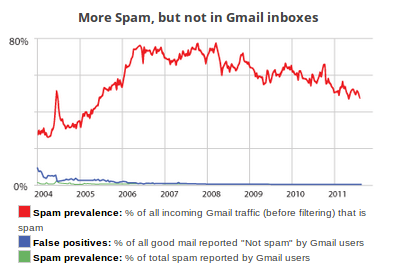
\includegraphics[height=5cm]{Imagens/gmail/spamchart.png} \footnote{Retirado de \url{http://www.google.com/mail/help/fightspam/spamexplained.html}}
	\end{figure}
\end{frame}

\section{Casos reais}
\subsection{Aviva Investors}
\begin{frame}{Aviva Investors}
	\begin{itemize}
		\item Administradora de fundo de investimentos globais
		\item E-mail de demissão enviado por engano para 1300 funcionários de 16 países
		\linebreak
		\item E-mail de retificação enviado 30 minutos mais tarde
	\end{itemize}
\end{frame}

\subsection{Coxinha em promoção}
\begin{frame}{Coxinha em promoção}
	\begin{itemize}
		\item Jornalista Lúcia Guimarães
		\begin{itemize}
			\item Mora em Nova Iorque
		\end{itemize}
		\item Recebe e-mail de uma promoção de um salgado
		\begin{itemize}
			\item Cidade Baixa de Porto Alegre
			\item 50\% de desconto
			\begin{itemize}
				\item De R\$12.50 por R\$6.00
			\end{itemize}
		\end{itemize}
		\item R\$4.000 a passagem para Porto Alegre
	\end{itemize}
\end{frame}

\subsection{Amizades via spam}
\begin{frame}{Amizades via spam}
	\begin{itemize}
		\item Início em 29 de fevereiro
		\item Um grupo de pessoas recebia e-mails
		\begin{itemize}
			\item Ao clicar em "responder", mesmo que apenas para o remetente, a mensagem era encaminhada para o grupo
		\end{itemize}
		\item Várias pessoas mandaram mensagens pedido, mandando e obrigando a tirá-los da lista de e-mails
		\begin{itemize}
			\item Sr. Clark chegou a mandar 12 mensagens em uma hora
			\item Acabou recebendo ligações de queixas de várias pessoas
		\end{itemize}
		\item Starwood Hotel era um dos integrantes da lista
		\begin{itemize}
			\item O hotel achou que as pessoas não queriam mais receber informativos do hotel
			\item Alguém acabou achando que a culpa era do hotel
			\item Chegou a ocorrer ameça envolvendo polícia italiana
		\end{itemize}
	\end{itemize}
\end{frame}

\begin{frame}{Amizades via spam}
	\begin{itemize}
		\item As pessoas perceberam que continuar respondendo só levaria a manter o ciclo de spam
		\item Um escritor de London sugeriu sairem para se encontrar, depois dessa onda de e-mails enviados
		\item Várias pessoas aderiram
		\item Grupo no \emph{LinkedIn}
		\begin{itemize}
			\item \emph{Unified by spam - the Social Experiment}
		\end{itemize}
	\end{itemize}
\end{frame}

\section{Estudo de caso}
\subsection{Apresentação do caso}
\begin{frame}{Estudo de caso}
\begin{itemize}
	\item Baseado em fatos
	\item Juliano
	\begin{itemize}
		\item Professor de uma Universidade renomada
		\item Ministra determinada disciplina num determinado semestre
	\end{itemize}
	\item Eduardo
	\begin{itemize}
		\item Pós-graduando sobre tutoria de Juliano
		\item Iminência de defender o mestrado
		\item Auxilia Juliano com a disciplina
	\end{itemize}
\end{itemize}
\end{frame}

\begin{frame}{Estudo de caso}
\begin{itemize}
	\item Média final da disciplina composta por projetos e nenhuma prova
	\begin{itemize}
		\item Projetos lançados ao longo do semestre
	\end{itemize}
	\item Testes são necessários pra comprovar eficiência e são realizados em máquinas específicas
	\item Máquina compartilhadas
	\begin{itemize}
		\item Flutuação do resultado
	\end{itemize}
\end{itemize}
\end{frame}

\begin{frame}{Estudo de caso}
	\begin{itemize}
		\item Alocação dos recursos feito pelo professor
		\begin{itemize}
			\item Horários não levavam em conta disponibilidade dos alunos
			\item Grupos não conseguiram terminar os testes
			\item Vários e-mails pedindo nova alocação
		\end{itemize}
		\item Juliano pede a Eduardo para mandar e-mails para os alunos avisando sobre as mudanças
		\item Eduardo faz o que foi pedido, mas percebe que ainda haverá várias mudanças
	\end{itemize}
\end{frame}

\begin{frame}{Estudo de caso}
\begin{itemize}
	\item O \emph{site} da disciplina poderia ser usado para avisar sobre as mudanças
	\begin{itemize}
		\item Apenas Juliano possuía acesso para realizar alterações
	\end{itemize}
	\item Os e-mails de modificações poderia ser mandado apenas para os grupos afetados
	\item Eduardo avisa Juliano que mandar a todos se trataria de um spam
	\begin{itemize}
		\item Juliano diz ser irrelevante
	\end{itemize}
\end{itemize}
\end{frame}

\subsection{Códigos da ACM violados}
\begin{frame}{Códigos da ACM violados}
		\begin{itemize}
			\item ``Contribuir para o bem-estar humano e da Sociedade''\\
				
			\item ``Procurar alcançar a maior qualidade, eficácia de dignidade tanto nos processos como nos produtos do trabalho profissional''\\
				
			\item ``Adquirir e manter competência profissional''\\
				
		\end{itemize}
\end{frame}

\begin{frame}{Grafo de obrigações}
	\begin{figure}
		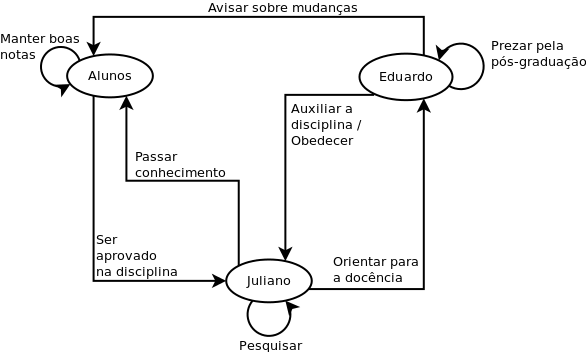
\includegraphics[height=5cm]{diagramas/grafo-de-obrigacoes.png}		
	\end{figure}
\end{frame}

\subsection{Obrigações, benefícios e vulnerabilidades}
\begin{frame}{Tabela de Obrigações}
	\begin{table}[h!]
		\centering
		\begin{tabular}{@{\extracolsep{\fill}} l C{0.2\textwidth} C{0.2\textwidth} C{0.2\textwidth}}
			\hline
								&	\textbf{Juliano}		&	\textbf{Eduardo}	&	\textbf{Alunos}\\	
			\hline
			\textbf{Juliano}	&	Pesquisar	&	Orientar para a docência	&	Passar conhecimento\\
			\hline
			\textbf{Eduardo}	&	Obedecer \linebreak \linebreak Auxiliar na disciplina	&	Prezar pela pós-graduação	&	Avisar sobre mudanças\\
			\hline
			\textbf{Alunos}	&	Ser aprovado na disciplina	&			&	Manter boas notas\\
			\hline
		\end{tabular}
	\end{table}
\end{frame}

\begin{frame}{Tabela de benefícios}
	\begin{tiny}
	\centering
		\begin{table}[h!]
			\centering
			\begin{tabular}{@{\extracolsep{\fill}}C{0.17\textwidth}  C{0.17\textwidth} C{0.17\textwidth} C{0.17\textwidth} C{0.17\textwidth} C{0.17\textwidth}}
				\hline
				 & \textbf{Insistir para Juliano modificar no site} & \textbf{Enviar apenas para os interessados} & \textbf{Enviar para todos} & \textbf{Enviar todas as modificações de uma vez}\\
				\hline
				Alunos interessados & Não receberão nenhum e-mail \linebreak \linebreak Serão notificados & Serão notificados & Serão notificados & Receberão menos e-mails \linebreak \linebreak Serão notificados\\
				\hline
				Alunos não interessados & Não receberão nenhum spam & Não receberão nenhum spam &  & Receberão menos e-mails\\
				\hline
				Eduardo & Não precisa enviar os e-mails & & & Envia menos e-mails \\
				\hline
				Juliano & & Não envia e-mails & Não envia e-mails & Não envia e-mails \\
				\hline
			\end{tabular}
		\end{table}
	\end{tiny}
\end{frame}

\begin{frame}{Tabela de vulnerabilidades}
	\begin{tiny}
		\begin{table}[h!]
			\centering
			\begin{tabular}{@{\extracolsep{\fill}}C{0.15\textwidth} C{0.15\textwidth} C{0.15\textwidth} C{0.15\textwidth} C{0.15\textwidth}}
				\hline
				& \textbf{Insistir para Juliano modificar o documento no site} & \textbf{Enviar apenas para os interessados} & \textbf{Enviar para todos} & \textbf{Enviar todas as modificações de uma vez}\\
				\hline
				Alunos interessados & & & Recebe spam & Recebe spam \\
				\hline
				Alunos não interessados & & & Recebe spam & Recebe spam \\
				\hline
				Eduardo & & Envia e-mails & Envia e-mails & Envia e-mails \\
				\hline
				Juliano & Precisa modificar o documento & & &\\
				\hline
			\end{tabular}
		\end{table}
	\end{tiny}
\end{frame}

\begin{frame}{Tabela de obrigações afetadas}
	\begin{tiny}
		\begin{table}
			\begin{tabular*}{\textwidth}{@{\extracolsep{\fill}} C{0.08\textwidth} | C{0.08\textwidth} C{0.08\textwidth} C{0.115\textwidth} C{0.115\textwidth} C{0.115\textwidth} C{0.115\textwidth}}
				\cline{2-7}
				& & & \textbf{Insistir para Juliano modificar no site} & \textbf{Enviar apenas para os interessados} & \textbf{Enviar para todos} & \textbf{Enviar todas as modificações de uma vez}\\
				\hline
				\multirow{3}{*}{Eduardo}  & Para ele mesmo & Prezar pela pós-graduação & - - & - - & - & - \\
				\cline{2-7}
						& Juliano & Obedecer & - & + & + + & + \\
				\cline{2-7}
						& Alunos & Notificar & + - & + & + & + \\
				\hline
				Juliano & Para ele mesmo & Pesquisar & - - &  &  & \\
				\hline
			\end{tabular*}
		\end{table}	
	\end{tiny}
\end{frame}

\subsection{Decisão consensual}
\begin{frame}{Decisão consensual}
	\begin{itemize}
		\item Eduardo tentar convencer Juliano a atualizar o site.
		\begin{itemize}
			\item Se a relação com o orientador ficar ruim, mandar as notivficações em blocos
		\end{itemize}
	\end{itemize}
\end{frame}


\section{Links interessantes}
\begin{frame}{Links interessantes}

	\begin{itemize}
		\item Yahoo Visualization Tool
		\begin{itemize}
			\item \url{http://visualize.yahoo.com/mail/}
		\end{itemize}
		\item Google Postini Services
		\begin{itemize}
			\item \url{http://www.google.com/postini/threat_network.html}
		\end{itemize}
	\end{itemize}

\end{frame}

\section{Referências}
\begin{frame}{Referências}
	\begin{itemize}
		\item [1] Monty Python, \emph{Spam}, 1970, \url{http://www.youtube.com/watch?v=anwy2MPT5RE} 
	\end{itemize}
\end{frame}

\end{document}